%%%%%%%%%%%%%%%%%%%%%%%%%%%%%%%%%%%%%%%%%%%%%%%%%%%%%%%%%%%%%%%%%%%%%%%%
%                                                                      %
%     File: Thesis_Implementation.tex                                  %
%     Tex Master: Thesis.tex                                           %
%                                                                      %
%     Author: Andre C. Marta                                           %
%     Last modified :  2 Jul 2015                                      %
%                                                                      %
%%%%%%%%%%%%%%%%%%%%%%%%%%%%%%%%%%%%%%%%%%%%%%%%%%%%%%%%%%%%%%%%%%%%%%%%

\chapter{SoC Design}
\label{chapter:socdesign}

\section{RISC vs CISC}
\label{section:riscvisa}

There are two types of ISAs: reduced and complex instruction sets. The desktop
PC market has been dominated by Intel's x86 ISA, a complex instruction set
architecture that was first introduced in 1978 as a 16-bit ISA. In 1985, the x86
ISA was expanded to 32-bit and in 2003 to 64-bit. However, in the embedded
systems market, companies like ARM gained the upper hand with reduced
instruction set processor core architectures in the 21\textsuperscript{st}
century.

\subsection{RISC and CISC definitions}
\label{subsection:risccisc definitions}

On the one hand, a reduced instruction set architecture is an ISA that provides
a small set of simple instructions that allow the machines they are implemented
in to have a reduced CPI (Cycles Per Instruction). These machines are called
Reduced Instruction Set Computers (RISC). On the other hand, as opposed to
reduced instruction sets, a complex instruction set architecture is an ISA were
each instruction sequence of several lower level operations (or
micro-operations) (for example, a memory load of one or more operands, an
arithmetic operation on these and a subsequent memory store of the result). The
machines that implement a complex instruction set are called Complex Instruction
Set Computers (CISC\footnote{The term CISC is usually used to refer to any
  non-RISC computer system. For example, a microcontroller that does not
  separate memory loads/stores from arithmetic operations can be labeled as
  CISC.}).

\subsection{Performance comparison between RISC and CISC ISAs}
\label{subsections:riscciscperformance}

CISC and RISC are two different approaches to tackle the performance problem in
CPUs. The performance of a benchmark program can be expressed as the inverse of
the time $t$ taken for the program's execution to complete, which in turn is
usually given by the Performance Equation in~(\ref{eq:performance}):

% Performance equation
\begin{equation}
\label{eq:performance}
t = N_I \cdot CPI \cdot T_{CLK} = \frac{N_I \cdot CPI}{f_{CLK}},
\end{equation}

where:

\begin{itemize}
	\item $N_I$ is the number of instructions of the benchmark program.
	\item $CPI$ is the average number of clock cycles per instruction;
	\item $T_{CLK} = \frac{1}{f_{CLK}}$ is the clock period (i.e. the duration of one clock cycle);
	\item $f_{CLK}   = \frac{1}{T_{CLK}}$ is clock frequency;
\end{itemize}

While the CISC approach, in order to increase performance, tries to reduce the
number of instructions $N_I$ sacrificing the number of clocks per instruction
(CPI), the RISC approach does the opposite: it reduces the CPI sacrificing
$N_I$.

% CISC performance
\subsubsection{CISC performance}
CISC architectures often have higher CPI values because the instructions are
usually multi-step sequences of simpler operations which take one clock cycle
each (or a few more), resulting in instructions that take several clock cycles
to execute. Because the instructions are built this way, they can be much more
specific and customizable. For this reason, CISC based ISAs have a huge number
of instructions, with many different sets of similar ones that differ only in
very specific details. This allows for an ISA to have a very complete set of
instructions, which results in extremely small and efficient assembly codes and,
therefore, the reduction of the number of instructions $N_I$ in programs.

% RISC performance
\subsubsection{RISC performance}
RISC ISAs, as it was said in Subsection~\ref{subsection:risccisc definitions},
are built so that its instructions are simple and executable in the minimal
number of clock cycles targeting low CPI values, as opposed to CISC ISAs. A
consequence of this feature is the increase of the programs' code size, as more
instructions are needed to perform the same operations done by CISC
instructions. This explains why $N_I$ in RISC ISAs are higher than in CISC ISAs.

% RISC and CISC debate is irrelevant nowadays
\subsubsection{RISC vs CISC performance conclusions}
As referred in~\cite{bib:ciscriscirrelevant}, the differences between the CISC
and RISC ISAs in performance were more important in the 1980's than in modern
times, because the key constraints back then were the chip area and the
processor design complexity. Nowadays, the primary constraints are low energy
and power consumption, where using RISC or CISC seems irrelevant; ARM's RISC
cores have penetrated the high-performance servers market (previously dominated
by Intel's x86 CISC cores) while Intel's x86 CISC cores have penetrated the mobile
low power devices market (previously dominated by ARM's RISC cores).

Also in \cite{bib:crisc} it is stated that the RISC vs CISC debate is of no more
interest nowadays, as it mentions that today's CISC CPUs (i.e. x86 CPUs) are not
true CISC cores anymore, but instead are CRISC (Complex-Reduced Instruction Set
Computer) cores, which means that they still execute the x86 CISC instruction
set, but their internal implementation is based in RISC principles. This means
that the internal behavior of both types of ISAs may not be so different, which
may justify why this choice does not affect performance.

% Brainiac microarchitecture designs influence performance greatly
According to~\cite{bib:ciscriscirrelevant}, the differences in performance
between the ARM Cortex-A8 and Cortex-A9 and Intel Atom and Sandybridge i7
microprocessors are due to the microarchitecture features of the various cores
such as:

\begin{itemize}
\item out-of-order execution;
\item instruction-level parallelism (i.e. superscalar processors); 
\item cache hierarchies and policies;
\item speculative execution (i.e. branch predictors);
\item data-level parallelism (i.e. vector processors);
\item register renaming;
\end{itemize}

The microarchitecture seems to have a significant impact on performance. In
particular, in the x86 cores manage to maintain high performance chiefly due to
the highly accurate branch predictor and large caches and not because of its
ISA. So, the conclusion is that the RISC vs CISC performance debate is
irrelevant nowadays.

\subsection{Advantages and disadvantages of RISC and CISC cores}
\label{subsections:riscciscadvantages}

Although performance is not an issue in the RISC vs CISC debate, there are other
factors that influence companies to opt for RISC cores instead of CISC cores in
their designs.

% CISC
\subsubsection{CISC}

Because there are no open source CISC cores available, a company would either
have to get an x86 core license from Intel, AMD or VIA Technologies (which are
the only companies in the world that manufacture x86 cores) or develop their own
x86 core. Both options are too expensive for small companies and developing an
x86 core has the extra cost of paying Intel a licensing fee, since they own the
x86 ISA.

But even if that licensing cost was covered, developing and maintaining a CISC
core and its toolchain is an overkill for smaller companies because both grow
much in complexity over time, which means that adding new features and
optimizing hardware and software will need more time and people. However, the
degree of complexity achieved in both the CISC core hardware and the compiler
(let alone the remaining toolchain components) is so high that the resources
needed at a certain point would be simply too much for a small company to
continue development and/or maintenance.

x86 is the only CISC ISA that survived along the years, and the only reason for
that to happen is the compatibility with older legacy systems. One can even
argue that pure CISC systems do not exist anymore, because like mentioned
before, today's x86 systems are CISC only on the outside, while their internal
implementation is RISC-based~\cite{bib:crisc}.

% RISC
\subsubsection{RISC}

A company has much better reasons for using a RISC core and much more options
available. The most obvious one is getting a licence from ARM to use one of
their proprietary RISC cores. It can use an open source RISC core available in
code sharing platforms like GitHub or BitBucket or it can even develop their
own, as there are many open and free RISC ISAs, being RISC-V the most prominent
one. From a resources point of view, a RISC core is the only option to even
consider, as the downsides of CISC are too much for even considering using it.

Besides, a RISC core has much ok foless hardware (and therefore less area and power
consumption) than a CISC one in small systems, because CISC needs much more
instruction decode logic due to the ISA's large number of instructions. The same
cannot be said for very high performance systems with much additional hardware
like caches, branch predictor, register renaming and others, as these will
occupy most of the chip's hardware and physical area and, therefore, will
dissipate much more power. However, these are not the kind of systems that are
targeted in this project, but instead the focus are low power and small area
SoCs and embedded systems for IoT applications.

Also, even if a more complex instruction set is needed, one can build it on top
of the open-source RISC-V ISA, as it support custom-made ISA extensions. With
the due skills and knowledge, one can even tweak the compiler's source code (as
it is open source) to account for pseudo-instructions that in truth consist of
sequences of real instructions that are actually contemplated in the RISC-V ISA,
mimicking CISC's instruction microcoding.





\section{The RISC-V ISA}
\label{section:riscvisa}

In the previous chapter, the reasons why RISC processors are more suited for SoC
development and embedded systems were described. Summarizing, RISC processors
generally need less hardware, occupy less area, consume less power and there are
free open source ISAs and respective cores available in GitHub and other alike
platforms. Indeed, most of the embedded system and SoC market consists of
RISC-based solutions.

The main free open source RISC ISA nowadays is RISC-V, a free reduced
instruction set architecture and surrounding software ecosystem that allows
standard and custom extensions of its base ISA. There are also other
alternatives for open source RISC ISAs such as OpenRISC, although it has few
commercial implementations.

\subsection{Brief History}

The RISC-V project started in 2010 at the University of California,
Berkeley. Since then, many contributors such as volunteers and industry workers
have joined the project, building a large RISC-V community. A startup called
SiFive was created in 2015 to encourage RISC-V dissemination in the
semiconductor and electronic design industries. On November 29, 2016, SiFive
released the first integrated circuit (IC) that implements the RISC-V ISA and in
October 2017 they released the first SoC that supports fully featured operating
systems (OSs) like Linux, which validates the RISC-V ISA's potential to become
an industry standard in the future.

In 2018, the RISC-V ISA continues to gain importance in the semiconductor IP
industry also for large companies like NVidia and Western Digital Corp., who
\textit{"have decided to use RISC-V in their own internally developed
  silicon. Western Digital's chief technology officer has said that in 2019 or
  2020, the company will unveil a new RISC-V processor for the more than 1
  billion cores the storage firm ships each year. Likewise, Nvidia is using
  RISC-V for a governing microcontroller that it places on the board to manage
  its massively multicore graphics processors"} \cite{bib:opinion}.

\subsection{Instruction set architecture}

The RISC-V ISA supports four base ISA and several standard extensions, whose
names and status can be consulted in Table~\ref{table:isa}. It is also possible
to build custom extensions for the RISC-V ISA like, for example, GPU-based
instruction sets.

\subsubsection{User-level ISA}
\label{subsection:userlevelisa}

At the time of writing of this document, the RISC-V user-level architecture is
in version 2.2. This current version of the RISC-V user-level architecture
manual \cite{bib:riscvmanual} contains the following versions of the RISC-V ISA
modules:

% Tabela: https://github.com/riscv/riscv-isa-manual/blob/master/src/preface.tex
\begin{table}[!htb]
\renewcommand{\arraystretch}{1.2} % more space between rows
\caption{The RISC-V user-level architecture, version 2.2 (taken from~\cite{bib:riscvmanual}, Preface, page i).}
	\centering
	\small
	\begin{tabular}{clc}
		\toprule
		Base     & Version & Frozen? \\
		\midrule
		RV32I    & 2.0 & Y \\
		RV32E    & 1.9 & N \\
		RV64I    & 2.0 & Y \\
		RV128I   & 1.7 & N \\
		\midrule
		Extension & Version & Frozen? \\
		\midrule
		M        & 2.0 & Y \\
		A        & 2.0 & Y \\
		F        & 2.0 & Y \\
		D        & 2.0 & Y \\
		Q        & 2.0 & Y \\
		L        & 0.0 & N \\
		C        & 2.0 & Y \\
		B        & 0.0 & N \\
		J        & 0.0 & N \\
		T        & 0.0 & N \\
		P        & 0.1 & N \\
		V        & 0.2 & N \\
		N        & 1.1 & N \\
		\bottomrule
	\end{tabular}
	\label{table:isa}
\end{table}

The currently defined extensions to the base Integer (I) ISA are:

\begin{itemize}
\item M, which provides integer multiplication and division instructions;
\item A, which provides atomic\footnote{Instruction that read and write in the
  same memory position in order to prevent other CPU core or I/O device to
  access it before the instruction is completed.} instructions;
\item F, D, and Q, which provide floating point operations in single (32-bit),
  double (64-bit) and quadruple (128-bit) precision, respectively;
\item C, which provides compressed instructions. 
\end{itemize}

The other expansions contemplated in Table~\ref{table:isa} are still in
development.

The standard ISA's instructions are all 32-bit wide. This results in a simple
implementation but in large code sizes, which, as pointed out in
Section~\ref{subsections:riscciscperformance}, typically happens in RISC
architectures. To mitigate this issue, the instructions were built to use, in
reality, only 30 bits, which allows for 3/4 of the opcode space to be used
to address a variable-length subset of instructions.

The two remaining bits of the instruction/opcode are used to select 3
subsets\footnote{There are 4 subset in total, corresponding to the four possible
  combinations of this 2-bit word. When at least one bit is 0, a compressed
  subset of only 16-bit wide instructions is used. All 32-bit instructions have
  both of these bits set to 1.} of smaller instructions (typically 16-bit
wide\footnote{When the base ISA used is RV64I or RV128I, these instruction do
  not necessarily use 16 bits, but usually half of the size of the base ISA's
  instructions.}), which are aliases of the larger base ISA's instructions. This
compressed instruction alias scheme is also used in other compressed RISC ISAs
like ARM's Thumb and the MIPS16.

However, RVC (RISC-V's compressed ISA) has an advantage over the previous two,
because it was built so that each of its compressed instruction expands into a
single 32-bit instruction in one of the base ISAs of the F and D standard
expansions, which lets regular and compressed instruction be used in a single
piece of code without having to worry about operation modes like in Thumb or
MIPS16.

Another advantage of this is that RVC instructions can be directly expanded in
the instruction decode stage, which accounts for less and simpler hardware. This
can make a RISC-V processor core much more efficient, as the instruction decode
hardware is usually one of the most (if not the most) costly energy consuming
parts of the processor circuit.

Having a compressed ISA also helps to reduce code size, because typically two
compressed instructions can fit in the same space as a regular instruction.

In conclusion, the compressed RISC-V ISA subset (C) is particularly useful for
embedded and SoC designs, because it allows for smaller code sizes and more
energy efficiency~\cite{bib:compressed}. Using the RV32E base ISA is also quite
useful in these kinds of systems, as it was made specially for them (the E stand
for "Embedded"). This base ISA uses only 16 32-bit integer registers (instead of
32 registers, like RV32I) and does not support floating point instructions
(although it is possible to use floating point software libraries). The RVC
extension is usually used alongside the RV32E base ISA in embedded systems and
SoCs.

\subsubsection{Privileged level ISA}
There is also a privileged level instruction set in the RISC-V
ISA~\cite{bib:riscvprivileged110}, which details privileged instructions and
other functionalities required for OS support and attaching external
devices. This part of the RISC-~V ISA is sill in the development stage and has
not yet been accepted by the RISC-V Foundation as standard.

\section{SoC structure}
\label{section:socdesign}

\subsection{SoC components}
A System on Chip (SoC) is an electronic system completely incorporated in a
single integrated circuit (or, as it is more simplistically often referred to, a
chip). Some components that make up an SoC are the same as those found in a
computer system such as CPU cores, memory units and several Input and Output
(I/O) ports and peripheral interfaces. Other typical components are
co-processors or peripheral modules that implement dedicated functions, such as
audio encoders or decoders, or even low power programmable hardware cores like
CGRAs (for example, Versat~\cite{bib:versat}).

The CPU is typically the key component of this kind of systems, because it is
where programs can be run. If a more specific task needs to be done, the CPU can
communicate with one of its dedicated peripherals or co-processors and feed them
with operands for they to process or receive their results.

If the SoC needs to receive external data or send data to the outside world, the
CPU can write or read to the I/O peripheral interfaces available in the SoC,
such as JTAG, Ethernet, USB, HDMI, UART, SPI, PCI Express and others. It is also
possible for an SoC to use interfaces for wireless communication protocols such
as WiFi and Bluetooth, although one needs to keep in mind that wireless
protocols may need support of lower layer devices, which may need to be external
chips due to their specificities.

An SoC typical structure is the one considered for building the \socname System
on Chip, which uses almost every type of component mentioned in the last
paragraphs. This structure is detailed in Subsection~\ref{section:mysoc}.

\subsection{SoC intermodule communication}

\subsubsection{Global bus infrastructure}
Traditionally, the various components that make an SoC communicate with each
other via a bus infrastructure that consists in a global shared bus. In order to
guarantee a certain throughput of data exchanges between the memory and other
components, Direct Memory Access (DMA) controllers can be used to bypass the
CPU, which cannot do these data transfers as fast and may be busy with other
things.

This kind of intermodule communication is not scalable, because when the number
of cores and/or components in an SoC rises above a certain level, the bus
infrastructure needed to ensure communication between all components grows to a
point where silicon area and power consumption are too high to meet the tight
specifications of IoT applications.

\subsubsection{Network on Chip}
A solution to this problem is implementing network structures based on Internet
protocols such as TCP and IP and routing algorithms such as Dijkstra's. This
approach is called Network on Chip (NoC). This not only greatly reduces the
silicon area occupied by wires connecting SoC modules and power consumption, but
also improves throughput and latency \cite{bib:noc}. Although this approach is
much more interesting than traditional bus communication infrastructures for IoT
applications, it also requires network knowledge such as communication protocols
and routing algorithms, as well as how these can be implemented in hardware
(routers). Besides, the \socname System on Chip will not have a large number of
components, so for now the traditional bus approach will be used. However,
implementing a NoC infrastructure in \socname is a very interesting perspective
for future work.

\section{The \socname System on Chip}
\label{section:mysoc}

\begin{figure}[!h]
\centering
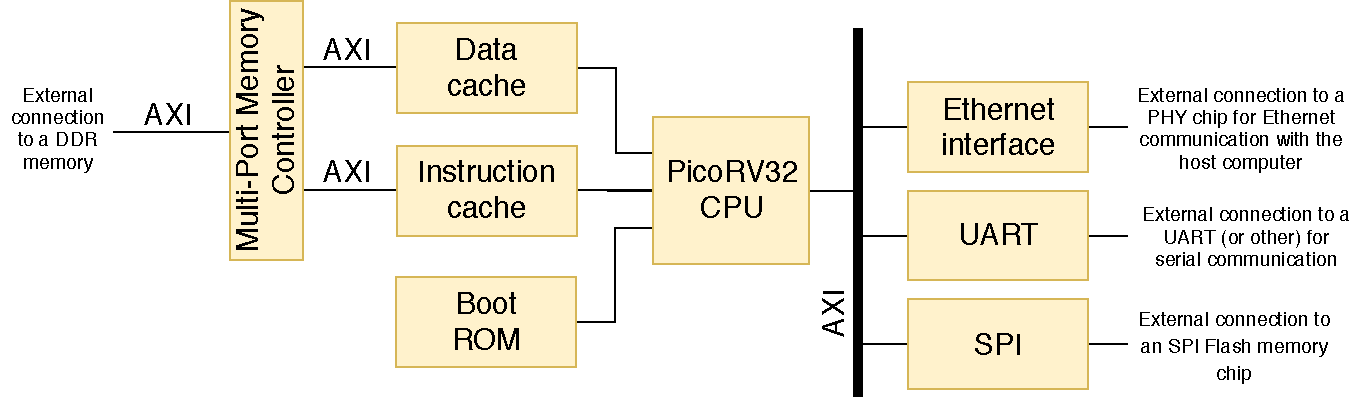
\includegraphics[width=1\linewidth]{Figures/soc2}
\caption{Top level block diagram of the \socname System on Chip.}
\label{fig:soc}
\end{figure}

The top-level topology of the \socname System on Chip is shown in
Figure~\ref{fig:soc}. \socname is intended to be build as a base SoC for future
development of IoT hardware and software systems, which means that the key
attributes of \socname must be small area, low power consumption and high
performance. Another very important feature for the \socname System on Chip and
for the development environment to be built during this project is
configurability, so to allow developers to choose which of the specifications
mentioned earlier are the most important to optimize, according to the
application intended for the SoC being developed.

As such, several RISC-V CPU alternatives were taken into account when choosing
which one of them was going to be used to build the \socname System on
Chip. Those were Rocket Chip \cite{bib:rocketchip}, Taiga \cite{bib:taiga},
PULPino \cite{bib:pulpino}, and PicoV32 \cite{bib:picorv32}. Brief descriptions
of each architecture are given next, as well as the identified reasons to
discard the ones that were not sufficiently fitting for the \socname System on
Chip.

\begin{itemize}
	
	\item \textbf{Rocket Chip} \cite{bib:rocketchip} is the de facto
          standard for SoC development using RISC-V processor cores, as it was
          made by the same team that introduced the RISC-V ISA. Rocket Chip is a
          synthesizable RTL generator that allows customization and
          parameterization of two RISC-V processor cores architectures (one
          being in-order and the other out-of-order). However, due to the fact
          that Rocket Chip has a great amount of features, it has proved to be
          too hard to manipulate in the past, so this option is put aside.
	
	\item \textbf{Taiga} \cite{bib:taiga} is a high-performance RISC-V
          softcore written in SystemVerilog, developed mainly for use in FPGAs
          and for supporting multicore configurations using an OS. However,
          given the fact that the focus of this architecture is to solely
          optimize performance and resource allocation in FPGAs, it not suited
          for the applications envisioned for this project, as the \socname
          System on Chip is meant to reach ASIC implementation.
	
	\item \textbf{PULPino} \cite{bib:pulpino} is an open source single core
          microcontroller system that can be configured to use either one of two
          different in-order and single-issue CPU architectures: RI5CY
          \cite{bib:riscy} or zero-riscy \cite{bib:zeroriscy}. Both are designed
          to be used in ultra low power \footnote{Ultra low power in eletronic
            circuits means that the transistors are operated with the minimal
            power supply possible. As such, the transistors are operated at
            sub-threshold regions, with ultra low threshold voltages.} designs
          \cite{bib:ultralowpower}.
	
	In particular, RI5CY has 4 pipeline stages, an IPC (Instructions Per
        Cycle) approximately equal to 1 \cite{bib:riscvmanual} and full support
        of the RV32I base instruction set. It supports some of the RISC-V ISA
        extensions, such as the RV32C, RV32M and RV32F and it also supports
        other ISA extensions such as fixed-point operations, dot product and
        others. RI5CY implements a subset of the privileged specification of the
        1.9 version of the RISC-V ISA~\cite{bib:riscvprivileged19}. As of the
        date of writing of this document, the latest version of the privileged
        architecture of the RISC-V instruction set is v1.10
        \cite{bib:riscvprivileged110}.
	
	The zero-riscy architecture is derived from RI5CY CPU core. It features
        2 pipeline stages and, like the RI5CY core, supports the RV32I base
        instruction set and the RV32C and RV32M extensions. It is also possible
        to reduce the number of registers to 16, configuring the zero-riscy core
        to adopt the RV32E RISC-V instruction set, which is useful for embedded
        systems. This architecture also implements a subset of the privileged
        specification of the 1.9 version of the RISC-V ISA, just like RI5CY.
	
	PULPino provides a set of peripherals such as I2S, I2C, SPI and UART for
        communication with external systems. PULPino, RI5CY and zero-riscy are
        were all written with the SystemVerilog HDL\footnote{SystemVerilog is
          also a Hardware Verification Language (HVL).} (Hardware Description
        Language).
	
	\item \textbf{PicoRV32} \cite{bib:picorv32} is a size-optimized RISC-V
          processor core that implements the RV32IMC instruction set. Although
          being small, it features a high maximum clock frequency (250-450 MHz
          on 7-Series Xilinx FPGAs, according to the README file in
          \cite{bib:picorv32}). The RV32C and RV32M extensions are supported, so
          it is possible to configure this PicoRV32 as an RV32IM, RV32IC or
          RV32IMC core. It is also possible to configure it as a RV32E core. It
          also supports other optional useful features for SoCs and embedded
          systems, such as a built-in interruption controller and a co-processor
          interface.
		
\end{itemize}

So, the two contenders for being the CPU architecture in the \socname System on
Chip are PULPino and PicoRV32. In the end, it was decided to use the PicoRV32
CPU architecture to build the \socname System on Chip. The reasons for choosing
this processor core over PULPino are the following:

\begin{enumerate}
	
\item PULPino's features, although interesting for SoC design and embedded
  systems, go beyond the scope of the project. Namely, it implements a subset of
  the RISC-V privileged ISA, which is a feature purposely left out of the
  project at hand because, for the time being, there is no interest in running
  an OS in the \socname System on Chip. Instead, a smaller set of simple custom
  instructions can be used for Interruption Request (IRQ) handling, which
  PicoRV32 already implements.

\item PicoRV32's GitHub repository is the most complete of the two, where there
  are made available some application examples of the PicoRV32 CPU, namely the
  PicoSoC example SoC and a simple system with just a CPU core and a memory unit
  connected by PicoRV32's native interface.

\item On the one hand, PicoRV32's provided testbenches in the respective GitHub
  repository delivered positive results. The simple CPU + memory system
  mentioned in the previous item was also synthesized in FPGA (details are in
  Chapter~\ref{chapter:results}). On the other hand, there were efforts in the
  past to integrate PULPino in a system being developed at IObundle, but the
  team was incapable of detaching the PULPino core from the environment where it
  was demonstrated because there was not enough information available to do so.

\end{enumerate}


%%%%%%%%%%%%%%%%%%%%%%%%%%%%%%%%%%%%%%%%%%%%%%%%%%%%%%%%%%%%%%%%%%%%%%%%
\subsection{CPU}
\label{subsection:cpu}

The CPU is the most important component of the system. It runs programs stored
in an external DRAM memory and connects to all other components\footnote{The CPU
  does not connect directly to the memory controller, but instead is connected
  through a cache interface.}.

The CPU architecture used in the \socname System of Chip is PicoRV32. It
supports the RVC standard RISC-V ISA extension and the base ISA RV32E, which are
important features for SoC development, as explained in
Subsection~\ref{subsection:userlevelisa}.

Other key features of PicoRV32 are:

\begin{itemize}
	\item Small size. When deployed on a 7-Series Xilinx FPGA, it uses
          between 750 and 2000 LookUp Tables (LUTs);
	\item Maximum frequency between 250 MHz and 450 MHz on 7-Series Xilinx
          FPGAs;
	\item CPI approximately equal to 4, but depends on the mix of
          instructions in the code. For more details, the README file
          in~\cite{bib:picorv32} should be consulted;
	\item Selectable native memory interface or AXI4-Lite master and Verilog
          description of an interface to use between two cores with different
          memory interfaces (AXI4-Lite or native);
	\item Optional IRQ support using a simple custom ISA;
	\item Optional Co-Processor Interface, which can be used to implement
          non-branching instructions in external co-processors, such as the M
          standard RISC-V ISA extension;
	\item Option to choose single-port or dual-port register file
          implementation, which can be useful to configure reduce the core's
          size or to increase it is performance;
\end{itemize}


%%%%%%%%%%%%%%%%%%%%%%%%%%%%%%%%%%%%%%%%%%%%%%%%%%%%%%%%%%%%%%%%%%%%%%%%
\subsection{Ethernet interface}
\label{subsection:ethernet}

Ethernet is a widely used communication protocol that was first commercially
introduced in 1980. Since then, it has evolved to a point where it is possible
to transfer data through Ethernet cables with bandwidths from 10 Mbit/s to 100
Gbit/s\footnote{Ethernet using more than 100 Gbit/s of bandwidth is called
  Terabit Ethernet (TbE). TbE standards for 200 Gbit/s and 400 Gbit/s Ethernet
  were developed by the IEEE P802.3bs Task Force and were approved on December
  6, 2017. However, the term Ethernet usually refers to the 10 Mbit/s to 100
  Gbit/s range, while the above ranges are referred as TbE.}. An Ethernet
interface is currently in development for a separate Versat~\cite{bib:versat}
project at IObundle, which is intended to be used in the \socname System on Chip
as well.

The Ethernet interface will be used instead of a JTAG tap for communication of
the \socname System on Chip with the host computer, with the objective of
reducing drastically the time needed to load programs into the SoC and to send
bitstreams from the host computers to FPGA where \socname is being emulated.

In the \socname System on Chip, the Ethernet interface will be connected to the
CPU via an AXI interface.


%%%%%%%%%%%%%%%%%%%%%%%%%%%%%%%%%%%%%%%%%%%%%%%%%%%%%%%%%%%%%%%%%%%%%%%%
\subsection{UART}
\label{subsection:uart}

An Universal Asynchronous Receiver-Transmitter (UART) is needed for debug and
printing purposes. A UART is a hardware device that implements the RS232 serial
protocol for data communication through two serial ports: one for transmitting
(often labeled as TX) and another for receiving (often labeled as RX). When data
transfer is taking place, the UART outputs a start byte in the TX port, followed
by the 8 bits that compose the byte that needs to be transmitted and finally a
stop bit. When receiving data, it checks if a start bit in the RX port in
received and, when detected, it receives the 8 bits and the stop bit and
converts the received serial data into a byte. So, the UART is usually used to
send char strings from the SoC to a terminal on the host computer. The UART also
has a clock divider scheme to adjust its BAUD rate.

The PicoRV32 GitHub repository already has an example SoC where a UART open
source Verilog description is included and connected to the CPU via the
PicoRV32's native memory interface. In the \socname System on Chip, the UART
will be connected to the CPU via an AXI interface.


%%%%%%%%%%%%%%%%%%%%%%%%%%%%%%%%%%%%%%%%%%%%%%%%%%%%%%%%%%%%%%%%%%%%%%%%
\subsection{SPI}
\label{subsection:spi}

A Serial Peripheral Interface (SPI) is also included to allow communication with
an SPI Flash memory unit, which can store program data destined to be transfered
to the CPU. However, the SPI can also be used to communicate with other low
speed peripherals. Similarly to the UART, the SPI is also a serial interface,
but while the UART transfers data asynchronously, the SPI offers synchronous
communication. The SPI is also much faster transferring data than the UART,
because the first can usually send data through 2, 3 or 4 wires, while the
second has only one wire available for this task.

An alternative to the SPI would be an I2C, which is also a synchronous serial
interface. However, there are numerous reasons why the SPI is preferable. The
most obvious one is that the I2C is typically slower and is more complex than
the SPI, because its hardware is based on an addressing scheme and the SPI
simply uses a chip select line. Also, SPI flash memory is the easiest and
cheapest kind of off-chip non-volatile memory available nowadays, so it is more
pertinent to consider an SPI.

The PicoRV32 GitHub repository already has an example SoC where an SPI open
source Verilog description is included and connected to the CPU via the
PicoRV32's native memory interface. In the \socname System on Chip, the SPI will
be connected to the CPU via an AXI interface.


%%%%%%%%%%%%%%%%%%%%%%%%%%%%%%%%%%%%%%%%%%%%%%%%%%%%%%%%%%%%%%%%%%%%%%%%
\subsection{Boot ROM}
\label{subsection:bootrom}

A Read-Only Memory (ROM) is typically used in computer systems to store a boot
program that is executed after each machine reset. As such, boot ROMs are
connected to the system's CPU. When the reset signal is received, it the boot
ROM loads the program to the CPU's memory and is then executed. During the
professional internship at IObundle, the author used the picoVersat controller
(i.e. Versat's~\cite{bib:versat} controller), where the boot program stored in
the boot ROM was a simple loop to check if a non-zero value was written to
register R0 (signaling that a program was ready to be executed) and, if it did,
a branch to the program memory's base address would be made, starting the
program.

In the \socname System on Chip, the boot ROM is connected to the CPU via
PicoRV32's native memory interface.


%%%%%%%%%%%%%%%%%%%%%%%%%%%%%%%%%%%%%%%%%%%%%%%%%%%%%%%%%%%%%%%%%%%%%%%%
\subsection{Multi-Port Memory Controller}
\label{subsection:memcontroller}

A DRAM controller is used to control data transfer between the external DRAM
memory and the CPU. The DRAM controller connects to the external DRAM memory and
to the data and instruction caches mentioned below through AXI interfaces, as
depicted in Figure~\ref{fig:soc}.


%%%%%%%%%%%%%%%%%%%%%%%%%%%%%%%%%%%%%%%%%%%%%%%%%%%%%%%%%%%%%%%%%%%%%%%%
\subsection{Instruction and Data Caches}
\label{subsection:caches}

Between the DRAM controller and the CPU, a data cache and an instruction cache
are present, in order to increase memory access performance. Caches are a kind
of smaller but faster memory used to interface a CPU and a RAM memory in order
to increase memory access speed. When the CPU access new data, it first checks
if the data is in the cache. If not, then the data is loaded from the RAM memory
to the cache so that the next time the processor needs to access it, it can read
or write it faster.

The caches are connected to the CPU via PicoRV32's native memory interface and
to the DRAM controller through an AXI interface.

